\subsection{System Description and Basic Assumptions}\label{sec:network:performance_model:system_description}

We consider a \gls{UE} which sends and receives a sequence of data packets via a \gls{3G} \gls{UMTS} network.
As discussed in \refsec{sec:network:background:umts_rrc}, the arrival process of the packet transmissions determines the \gls{RRC} states of the \gls{UE}.
However, the direction of packets, i.e. them originating from the \gls{UE} or the \gls{NodeB}, has no impact on the \gls{RRC} states, as the states depend solely on traffic activity.
Due to the high impact of \gls{RRC} states on traffic patterns, we do not consider packet sizes in this model.
In real \gls{UMTS} networks very small packets might be treated differently for \gls{RRC} states, but we neglect this both for simplicity reasons and because the impact of packet sizes is highly network operator specific~\cite{Qian2010a}.
Furthermore, \gls{RRC} state transitions are complex procedures depending on implementation details of the \gls{UE}, the specific \gls{UMTS} release, and the configurations by the network operator.
In order to keep our model simply, but realistic, we reduce the set of standardized \gls{RRC} states and the state transition triggers in the following ways. 

\begin{figure}
	\begin{subfigure}[b]{.5\textwidth}
	\centering
	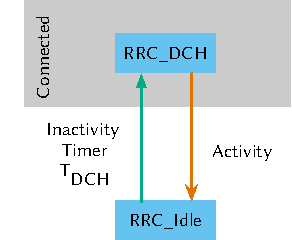
\includegraphics{network/background/figures/two_states}
	\caption{Two State Scenario}\label{fig:network:performance_model:system_description:rrc_state_machines:two_states}
	\end{subfigure}	\begin{subfigure}[b]{.5\textwidth}
	\centering
	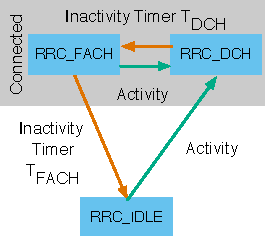
\includegraphics{network/background/figures/three_states}
	\caption{Three State Scenario}\label{fig:network:performance_model:system_description:rrc_state_machines:three_states}
	\end{subfigure}
	\caption{\headershortacr{RRC} State Machine Diagrams}\label{fig:network:performance_model:system_description:rrc_state_machines}
\end{figure}

In a first step we consider only a basic scenario with two \gls{RRC} states: \gls{RRC_idle} and \gls{RRC_DCH} as shown in \reffig{fig:network:background:rrc_state_machines:two_states}.
The \gls{UE} switches to \gls{RRC_DCH} to transmit or receive data and after an inactivity period of duration \gls{TDCH} it switches back to \gls{RRC_idle}. 
The motivation for the two states \gls{RRC} scenario is twofold.
First, it serves for illustration purposes.
We derive the model step-by-step in this simple scenario to explain the ideas behind the equations.
Then, the ideas can be easily transferred to the more complex three states scenario (cf. \refsec{sec:network:performance_model:system_description:three_states}).
Second, the scenario is of practical relevance since proprietary implementations of the fast dormancy concept \cite{NSN2011} exist, where the \gls{UE} decides to switch to \gls{RRC_idle} shortly after the transmission of a packet without using any other \gls{RRC} state.
Furthermore, this model is very similar to the one found in \gls{LTE} systems.
In \gls{LTE}, only a distinction between connected and disconnected states can be found, which maps to the \gls{RRC_idle} and \gls{RRC_DCH} states discussed in this model.

In our model we aggregate both packets sent and received by the \gls{UE} in in the packet arrival process, which is assumed to be a renewal process, i.e. a process  with identical and independently distributed inter-arrival times, described by the random variable \gls{PacketIAT} as shown in~\reffig{fig::twoStateModel}.
Thus, the probability that the time between two consecutive packets is at most \(t\) is \(P(\gls{PacketIAT} \leq t) = \gls{PacketIAT}(t)\).
We challenge this assumption by studying measurements of packet traces in \refsec{sec:network:performance_model:validations}.

The packet arrivals determine the \gls{RRC} state of the \gls{UE} and the corresponding transitions. Therefore, the packet arrival process can be seen as a modulating process, c.f. \cite{TranGia1983,TranGia1988}, while the state and the signaling process represent modulated, i.e., resulting processes.

\begin{figure}
  \centering
  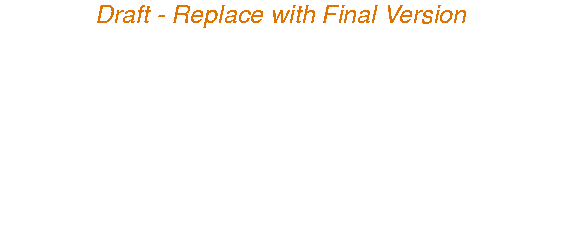
\includegraphics{network/performance_model/system_description/figures/arrival_process}
  \caption{Relation of Packet Arival Process \acrshort{PacketIAT}, State Process, and Signaling Process in the Two State Scenario}
  \label{fig:network:performance_model:system_description:arrival_process}
\end{figure}

\subsubsection*{The Case of Two \headershortacr{RRC} States}\label{sec:network:performance_model:system_description:two_states}

\newcommand{\RRCStateRealization}{\ensuremath{s}}
\newcommand{\ObservationInterval}{\ensuremath{T_{\text{Obs}}}}
\newcommand{\ObservationPoint}{\ensuremath{t^*}}
\newcommand{\ObservationIntervalDensity}{\ensuremath{q}}
\newcommand{\ObservationIntervalLength}{\ensuremath{\tau}}

\paragraph*{State Distribution:}
First, we are interested in the state distribution \(P(\gls{RRCState}=\RRCStateRealization)\), i.e., the fraction of time the \gls{UE} spends in state \(\RRCStateRealization\in\{\gls{RRC_idle},\gls{RRC_DCH}\}\) for a given inter-packet time \(\gls{PacketIAT}\).
For this purpose, we define an observation interval \ObservationInterval, depicted in \reffig{fig:network:performance_model:system_description:arrival_process}, which is assumed to be larger in orders of magnitude than the average packet inter-arrival time \(E[\gls{PacketIAT}]\).
In addition, we take the position of an outside observer who observes the state \gls{RRCState} at a random point in time \(\ObservationPoint\), uniformly distributed within the observation interval. 
Then the state distribution \(P(\gls{RRCState}=\RRCStateRealization)\) is the probability that the observer encounters the \gls{UE} in state \gls{RRCState} at the time \ObservationPoint. 

We calculate this distribution as 
\begin{equation}
P(\gls{RRCState}=\RRCStateRealization)= 
  \int_{0}^\infty \ObservationIntervalDensity(\tau) \cdot 
  P(\gls{RRCState}=\RRCStateRealization) \vert \gls{PacketIAT} = \ObservationIntervalLength) d\ObservationIntervalLength ,
  \label{eq::statedistribution} 
\end{equation} 
where \(\ObservationIntervalDensity(\ObservationIntervalLength)\) is the probability density that \ObservationPoint falls into an interval of length \(\ObservationIntervalLength\) and \(P(\gls{RRCState}=\RRCStateRealization) \vert \gls{PacketIAT} = \ObservationIntervalLength)\) is the probability that the UE is in state \gls{RRCState} under the condition that \ObservationPoint is within an interval of length (\ObservationIntervalLength\).


First, we derive \(\ObservationIntervalDensity(\ObservationIntervalLength)\). 
This probability density has to be proportional to $a(\tau)$ and to \ObservationIntervalLength, where $a(\ObservationIntervalLength)$ is the probability density function of the random variable \(\gls{PacketIAT}\). 
Therefore, we have that $\ObservationIntervalDensity(\ObservationIntervalLength)=a(\ObservationIntervalLength)\cdot\ObservationIntervalLength\cdot c_0$ with the proportionality constant $c_0$.\tabularnewline
Due to $\int_0^\infty \ObservationIntervalDensity(\ObservationIntervalLength)d\tau=1$, we have $c_0=1/E[\gls{PacketIAT}]$, which leads to
\begin{equation}
\ObservationIntervalDensity(\ObservationIntervalLength)=\frac{a(\ObservationIntervalLength) \cdot \ObservationIntervalLength}{E[\gls{PacketIAT}]}.
\label{eq::pdensObservation}
\end{equation}


\subsubsection*{Extension for Three \headershortacr{RRC} States}\label{sec:network:performance_model:system_description:three_states}
\subsubsection*{Modeling Signaling Intensity and Power Drain of the \headershortacr{UE}}\label{sec:network:performance_model:system_description:metrics}